\begin{figure}
\centering
  \begin{subfigure}[b]{28mm} 
    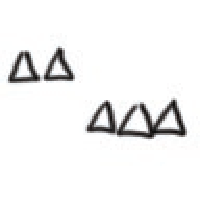
\includegraphics[width=\textwidth]{img/gestalt-proximity.pdf} 
    \caption{Proximity}
    \label{fig:gestalt-proximity}
  \end{subfigure}
  \hspace{2mm}
  \begin{subfigure}[b]{28mm} 
    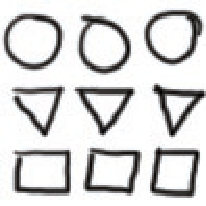
\includegraphics[width=\textwidth]{img/gestalt-similarity.pdf} 
    \caption{Similarity}
    \label{fig:gestalt-similarity}
  \end{subfigure}
  \hspace{2mm}
  \begin{subfigure}[b]{28mm} 
    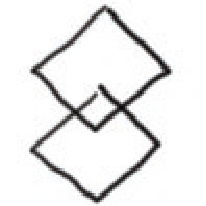
\includegraphics[width=\textwidth]{img/gestalt-symmetry.pdf} 
    \caption{Symmetry}
    \label{fig:gestalt-symmetry}
  \end{subfigure}
  \hspace{2mm}
  \begin{subfigure}[b]{28mm} 
    
\includegraphics[width=\textwidth]{img/gestalt-continuation.pdf} 
    \caption{Continuation}
    \label{fig:gestalt-continuation}
  \end{subfigure}
  \hspace{2mm}
  \begin{subfigure}[b]{28mm} 
    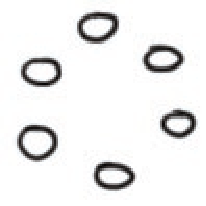
\includegraphics[width=\textwidth]{img/gestalt-closure.pdf} 
    \caption{Closure}
    \label{fig:gestalt-closure}
  \end{subfigure}
  \caption[Gestalt perceptual organization]{Some principles of
    perceptual organization~\cite{kanizsa-gestalt}.
    (\subref{fig:gestalt-proximity}) Proximity: elements near one
    another are seen as belonging to a
    group. (\subref{fig:gestalt-similarity}) Similarity: objects
    sharing features such as shape belong in the same
    group. (\subref{fig:gestalt-symmetry}) Symmetry: two shapes
    symmetric about horizontal and vertical axes, suggesting they
    belong together. (\subref{fig:gestalt-continuation}) Continuation:
    the simplest explanation is two straight lines, not four lines
    meeting in the middle. (\subref{fig:gestalt-closure}) Closure: A
    large circle emerges from an arrangement of smaller circles.}
  \label{fig:gestalt}
\end{figure}
